\documentclass[runningheads]{llncs}

% Official ECCV 2026 camera-ready style (final mode is the default).
\usepackage{eccv}
\usepackage{eccvabbrv}

\usepackage{graphicx}
\usepackage{lmodern}
\usepackage{booktabs}
\usepackage{tabularx}
\usepackage{array}
\usepackage{multirow}
\usepackage{microtype}
\usepackage{flafter}
\usepackage{enumitem}
\usepackage[accsupp]{axessibility}
\usepackage{hyperref}
\hypersetup{hidelinks,pdftitle={KoreaDrive: A System-Level Capability Analysis of Video-Language Understanding across TAR, FETV, and PSI-VQA at AI City Challenge 2026},pdfauthor={Hyunwoo Kim, Yooseung Wang, Pusik Park}}

\newcommand{\tar}{TAR\xspace}
\newcommand{\fetv}{FETV\xspace}
\newcommand{\psivqa}{PSI-VQA\xspace}
\newcommand{\qwen}{Qwen3-VL-8B-\allowbreak Instruct\xspace}
\newcolumntype{L}[1]{>{\raggedright\arraybackslash}p{#1}}
\newcolumntype{R}[1]{>{\raggedleft\arraybackslash}p{#1}}
\newcolumntype{Y}{>{\raggedright\arraybackslash}X}

\begin{document}

\title{KoreaDrive: A System-Level Capability Analysis of Video-Language Understanding across TAR, FETV, and PSI-VQA at AI City Challenge 2026}
\titlerunning{KoreaDrive: Capability Analysis across TAR, FETV, and PSI-VQA}

\author{Hyunwoo Kim \and Yooseung Wang \and Pusik Park\thanks{Corresponding author.}}
\authorrunning{H. Kim, Y. Wang, and P. Park}
\institute{Korea Electronics Technology Institute (KETI), Republic of Korea\\
\email{\{hwkim3, yswang, pusik.park\}@keti.re.kr}}

\maketitle
\begin{abstract}
Track 3 of the 2026 AI City Challenge evaluates traffic-video reasoning across Traffic Anomaly Reasoning (TAR), Fisheye Traffic Violation Understanding (FETV), and Pedestrian Situated Intent VQA (PSI-VQA). KoreaDrive applies deterministic task-specific frame, prompt, output-contract, parsing, and optional calibration controls to one frozen \qwen Vision-Language Model (VLM) backbone; no task-specific parameter update or adapter generated the leaderboard submissions. The three scored runs use the same model identifier, bf16 precision, visual budget, and recovered weight revision, establishing a common frozen checkpoint across the three evaluations. Public-board scores were 0.4256 on TAR, 0.4634 on FETV, and 57.04 on PSI-VQA. Controlled analyses show a task-dependent picture: explicit red-box grounding raises the routed PSI Multi-Choice Question (MCQ) configuration from 3/24 to 9/24 and is statistically indistinguishable from the 8/24 generic prompt; the video-aware temporal configuration improves over random intervals, and fitted metadata priors provide additional localization strength. A submission-artifact comparison further associates the largest late FETV gain with deterministic description formatting and timestamp handling, not with an isolated prompt change. On the TAR General board, the same KoreaDrive artifact is 0.1113 above the organizer baseline labeled Qwen3-VL-8B-Instruct, an external same-model-label reference whose exact configuration is unavailable.
\keywords{Traffic domains \and Vision-language model \and Video-language understanding \and Capability analysis \and AI City Challenge}
\end{abstract}

\section{Introduction}
Traffic-video reasoning requires more than event recognition. A useful system must bind questions to the correct target entity, follow that entity through time, infer causal and spatial relations, localize relevant intervals, and emit answers that satisfy heterogeneous evaluation contracts. The 10th AI City Challenge formalizes these demands through benchmarks spanning CCTV, fisheye intersection, and egocentric driving video~\cite{aicity2026track3,tang2026aicity}.

This paper describes KoreaDrive (Team 277; registered as \emph{Korea Drive} on the evaluation portal) across all three Track 3 evaluations: in-domain Traffic Anomaly Reasoning (\tar), out-of-domain Fisheye Traffic Violation Understanding (\fetv), and out-of-domain Pedestrian Situated Intent VQA (\psivqa). 
A single frozen \qwen checkpoint is shared across the three evaluations. Task-specific control selection changes only the frame policy, prompt program, generation budget, output contract, parser, and optional calibrator. The scored artifacts use bf16, up to 16 frames, 151,200 pixels per frame, and the recovered Qwen3-VL weight revision. %
The analyses show a task-dependent picture: explicit target grounding materially improves the routed PSI MCQ configuration, the shipped routed prompt does not outperform a generic prompt, the video-aware temporal model captures signal beyond random intervals while simple fitted priors remain competitive, and output-contract handling can determine whether useful visual evidence becomes a valid benchmark answer. These analyses complement the leaderboard results and separate shared-backbone capability from task-specific control effects.

The main findings are:
\begin{enumerate}[leftmargin=*,itemsep=2pt]
    \item \textbf{TAR:} the public-board score is 0.4256 (24th of 27). The same KoreaDrive submission appears on the separate TAR General board at 0.4256, which is 0.1113 above the organizer baseline labeled Qwen3-VL-8B-Instruct (0.3143) and above 11 of the 13 organizer baselines; the strongest organizer baseline, Cosmos3-Super, scores 0.5729. Because the organizer run exposes only a model label, it is an external same-model-label reference rather than a controlled same-checkpoint ablation.
    \item \textbf{FETV:} KoreaDrive ranks 3rd of 8 on the public leaderboard with 0.4634. The description score is second-highest on that board, and field-level analysis shows a clear split between strong global or overlay-associated attributes and lower-scoring violator-centric geometry and violation fields. Between submitted artifacts \texttt{v6\_fewshot} and \texttt{v7}, the score rises from 0.4238 to 0.4584 while the ten non-temporal structured fields remain unchanged; description formatting and date/time handling move jointly.
    \item \textbf{PSI-VQA:} KoreaDrive ranks 5th of 7 on the public leaderboard with 57.04. OpenQA reaches 0.6019, above the top-ranked team's 0.5833, and temporal mIoU reaches 0.5708, within 0.0043 of the fourth-place team.
    \item \textbf{Component analysis:} adding explicit red-box re-localization to the routed prompt raises PSI MCQ from 3/24 (routed alone) to 9/24, statistically indistinguishable from the 8/24 generic (no-routing) baseline; TAR question-window sampling changes a matched 25-item comparison from 15/25 to 16/25; and temporal calibration quantifies how much performance is provided by video evidence versus fitted metadata priors.
\end{enumerate}
Across the three tasks, we release the scored submission artifacts, configuration records, validators, controlled analyses, and provenance limitations needed to reproduce the reported analysis.

\section{Related Work}
\paragraph{Driving video question answering and reasoning.}
Autonomous-driving VQA has progressed from templated scene questions to video-based explanation and multi-step reasoning. NuScenes-QA combines camera and LiDAR context with 460K question-answer pairs~\cite{nuscenesqa}. LingoQA contains short driving videos and evaluates truthful free-form answers~\cite{lingoqa}. DriveLM represents perception, prediction, and planning as graph-structured VQA~\cite{drivelm}, while Reason2Drive emphasizes chain-based, interpretable driving reasoning~\cite{reason2drive}. Track 3 differs by evaluating one system across CCTV anomaly reasoning, fisheye violation records, and target-pedestrian intent under independent metrics.

\paragraph{Traffic and pedestrian datasets.}
The AI City Challenge has expanded from detection and tracking toward language-centric traffic understanding~\cite{aicity2024,tang2026aicity}. FishEye8K demonstrates the geometric difficulty of radial distortion and nonuniform resolution~\cite{fisheye8k}. PSI provides socially situated pedestrian behavior for autonomous driving~\cite{psi}; PSI-VQA reformulates this setting as binary, open-ended, multiple-choice, and temporal video QA. These domains require persistent identity and geometry beyond global language description.

\paragraph{Video-language backbones and structured generation.}
Qwen3-VL supports native video input, long context, and text-based temporal alignment~\cite{qwen3vl}. In this paper, \emph{frozen submission} means that no task-specific parameter update, adapter, or checkpoint modification was applied when generating the submitted predictions; adaptation was limited to inference-time prompts, sampling policies, generation budgets, parsers, vocabulary normalization, and calibration. We reserve \emph{official} for challenge-defined metrics, scorers, and board results; our own files and execution path are called \emph{scored submission artifacts} and the \emph{leaderboard-submission pipeline}. Our parser-and-fallback design is weaker than token-level constrained decoding: PICARD rejects invalid tokens through incremental parsing~\cite{picard}, and grammar-constrained decoding guarantees formal output structures without task-specific fine-tuning~\cite{gcd}. The observed missing-answer failures motivate replacing post-hoc extraction with such decoding-time constraints where model APIs permit them.

\section{Task Description}
\subsection{Traffic Anomaly Reasoning (TAR)}
The TAR test set contains 960 questions over 80 CCTV clips. Nine task components contribute to the official mean: binary-choice question (BCQ), multiple-choice question (MCQ), binary-choice open-ended (BCQ-OE), multiple-choice open-ended (MCQ-OE), open QA, causal linkage, scene description, temporal description, and video summarization. Temporal localization remains in the released test interface but is excluded from the official mean following the organizer's July 1 update~\cite{aicity2026track3}. Exact-choice tasks require normalized answer extraction, while open-ended tasks are evaluated with BERTScore-F1~\cite{bertscore}.

TAR therefore combines classification-like decisions with long-form generation in one submission file. A participant system must preserve the item identifier and emit task-compatible text for all task types; this heterogeneity motivates the shared routing interface described in \Cref{sec:system} rather than a single prompt and decoder contract.

\subsection{Fisheye Traffic Violation Understanding (FETV)}
FETV contains 200 fisheye intersection clips and is submitted through the evaluation server as Track 7, the first out-of-domain evaluation of Track 3~\cite{aicity2026track3}. Each JSON record includes a free-text description and structured fields for date, time, violation type, violator type, color, initial/final position, initial/final lane, intersection type, weather, and lighting. The description metric combines normalized CIDEr~\cite{cider} and BERTScore; the final score is
\begin{equation}
S_{\mathrm{FETV}}=0.25\,\mathrm{CIDEr}_{\mathrm{norm}}+0.25\,\mathrm{BERTScore}+0.5\,\mathrm{MacroF1}.
\end{equation}
Position uses a 3$\times$3 center-square convention, while lane indices are relative to the violator's direction of travel. In contrast to TAR, one FETV prediction couples global scene attributes, violator identity, geometry, and free-form language in a single structured record, making schema validity and violator consistency central to the submission.

\subsection{Pedestrian Situated Intent VQA (PSI-VQA)}
PSI-VQA is submitted through the evaluation server as Track 8, the second Track 3 out-of-domain evaluation~\cite{aicity2026track3}. It uses 40 egocentric clips and four subtasks: binary crossing-intent classification, cue-style OpenQA, multiple-choice cue identification, and temporal localization of the driver-decision-critical interval. Cue answers are matched using sentence embeddings~\cite{sbert}; the final score equally weights the four normalized task scores.

Each PSI subtask has a distinct output contract: Yes/No text, cue lists, a single MCQ letter, or a temporal JSON interval. This separation lets us analyze semantic evidence, answer control, and calibration independently in \Cref{sec:controlled}.

\begin{figure}[t]
\centering
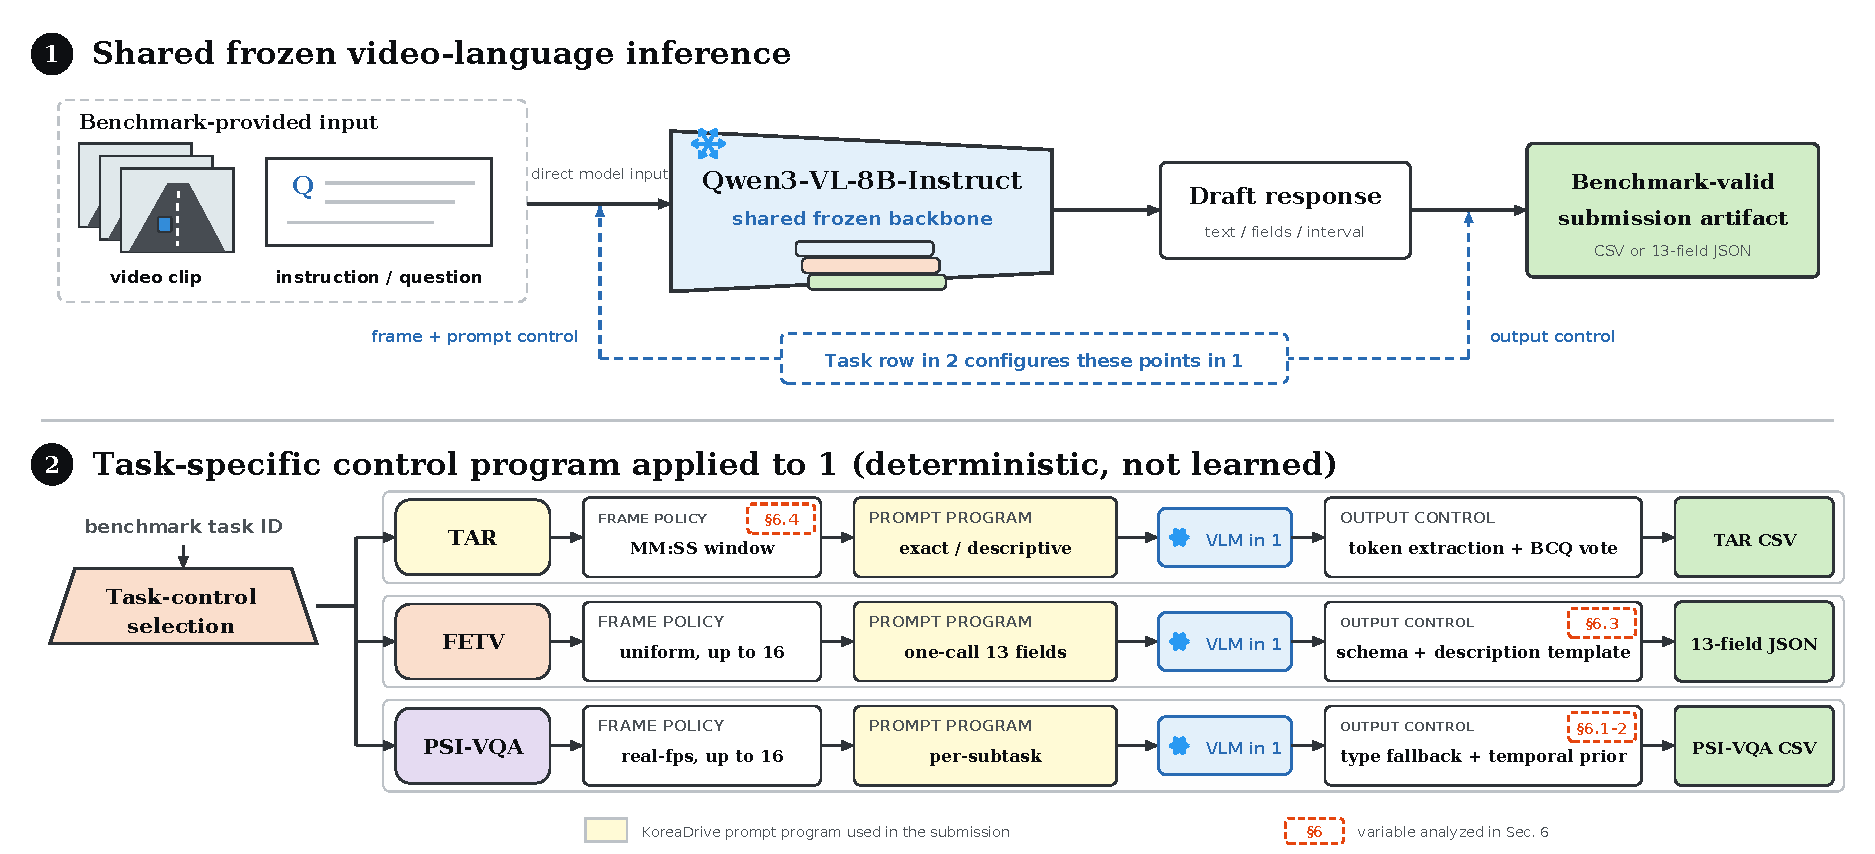
\includegraphics[width=\textwidth]{fig_system_overview.pdf}
\caption{Architecture of the KoreaDrive leaderboard-submission pipeline. Benchmark-provided video and instructions enter one shared frozen Qwen3-VL-8B-Instruct backbone directly. A deterministic, non-learned task selector configures the frame, prompt, and output-control program for TAR, FETV, or PSI-VQA; no task-specific adapter is used. Pale-yellow boxes identify prompt programs used in the scored submissions, and orange tags link the corresponding variables to Sec.~6 analyses.}
\label{fig:system}
\end{figure}

\section{KoreaDrive System}\label{sec:system}
\subsection{Shared backbone and task-specific control}
KoreaDrive uses one frozen VLM backbone for all three Track 3 evaluations. 
For each item, task-specific control selection chooses the frame-sampling policy,
prompt program, token budget, output contract, parser, and optional calibrator;
routing is implemented as deterministic control logic rather than a learned
router. The model then performs video-language generation, after which
benchmark-specific post-processing normalizes legal labels, extracts final
answers, validates schemas, or applies temporal calibration. Runners write
records incrementally, resume after interruption, and validate item coverage
before upload.

\Cref{fig:system} makes the two control paths explicit: benchmark-provided video and instructions feed the shared backbone directly, while the selector configures task-specific control modules around that backbone. All three scored artifacts use \qwen in bf16 at revision \texttt{0c351dd01ed87e9c1b53cbc748cba10e\allowbreak 6187ff3b}, with at most 16 frames and 151,200 pixels per frame. TAR uses question-window sampling and exact-choice or descriptive prompts; FETV generates one complete 13-field record; PSI-VQA selects subtask programs, type-correct extraction, and a duration-stratified prior. Yellow fill is descriptive and does not assert an aggregate prompt-only gain; measured effects are confined to the orange-tagged analyses in Sec.~6.


\subsection{Output contracts and validation}
BCQ and MCQ prompts request a normalized final token; temporal predictions request bare JSON; FETV requests a fixed schema. Parsers strip explanatory text, normalize vocabulary, and substitute type-correct fallbacks when parsing fails. These mechanisms ensure valid submission files but do not by themselves guarantee contract compliance. Using all available held-out generations per condition, 7/47 routed, 6/24 generic, and 4/24 box-aware outputs omitted a parseable final letter. The accuracy analysis in Sec.~6.2 instead uses only the 24 items common to all three conditions. These deliberately ambiguous training examples are not estimates for the official test set; they show why decoding-time answer control matters.

\subsection{Task programs}
For TAR, exact-choice prompts request short reasoning followed by a final token, while descriptive tasks receive longer budgets. For FETV, one call predicts the complete 13-field record, after which illegal fields and surface variants are normalized and the final description template is constructed. The submitted FETV pipeline does not include a detector, tracker, lane segmenter, or standalone OCR module. For PSI-VQA, cue answers are shortened to independently verifiable observations and task-specific parsers enforce the required answer type. The temporal submission uses a duration-stratified rule,
\begin{equation}
\hat I(d)=\begin{cases}\left[0.30d,0.70d\right],&d<10\ \mathrm{s},\\ \left[0.20d,0.62d\right],&d\ge10\ \mathrm{s}.\end{cases}
\end{equation}
with integer-second endpoints. These shipped constants were fitted on all 227 released training intervals; \Cref{sec:temporal} evaluates the same design under held-out refitting.

\section{Leaderboard Results}
\subsection{Leaderboard summary}
The portal maintains separate public and general boards. All ranks in the paper refer to the public board. \Cref{tab:overall} lists the scored submission artifacts and denominators. The leaderboards are independent and their scores are not combined.

\begin{table}[!ht]
\caption{Organizer-scored public-board results and archived submission artifacts.}
\label{tab:overall}
\centering
\small
\begin{tabularx}{\textwidth}{@{}L{0.14\textwidth}L{0.15\textwidth}L{0.13\textwidth}Y@{}}
\toprule
Evaluation & Public rank & Score & Submitted artifact \\
\midrule
TAR & 24 of 27 & 0.4256 & \texttt{submission\_qwen3vl8b\_v9.csv} \\
FETV & 3 of 8 & 0.4634 & \texttt{fetv\_submission\_v11.json} \\
PSI-VQA & 5 of 7 & 57.0400 & \texttt{psi\_vqa\_submission\_v7.csv} \\
\bottomrule
\end{tabularx}
\end{table}

\subsection{Traffic Anomaly Reasoning (TAR)}

\begin{table}[t]
\caption{Complete TAR component scores. Temporal localization was reported but excluded from the official mean.}
\label{tab:tar}
\centering
\small
\begin{tabular}{@{}lr@{\qquad}lr@{}}
\toprule
Task type & Score & Task type & Score \\
\midrule
BCQ accuracy & 0.5437 & Open QA F1 & 0.3333 \\
MCQ accuracy & 0.5875 & Causal linkage F1 & 0.2874 \\
BCQ-OE BERTScore-F1 & 0.4824 & Scene description F1 & 0.3282 \\
MCQ-OE BERTScore-F1 & 0.7664 & Temporal description F1 & 0.1856 \\
Video summarization F1 & 0.3160 & Temporal localization mIoU$^*$ & 0.1990 \\
\bottomrule
\multicolumn{4}{l}{\scriptsize $^*$Excluded from the mean after the 2026-07-01 rule update.}
\end{tabular}
\end{table}


\begin{table}[t]
\caption{Complete FETV public leaderboard (200-clip full test set). KoreaDrive denotes Team 277, registered on the evaluation portal as ``Korea Drive.''}
\label{tab:fetvleader}
\centering
\scriptsize
\begin{tabular}{@{}clrrr@{}}
\toprule
Rank & Team & Final & Description & Categorical mean \\
\midrule
1 & UWIPL\_ETRI & 0.4891 & 0.4171 & 0.5612 \\
2 & MR-CAS & 0.4884 & 0.4411 & 0.5358 \\
3 & KoreaDrive & \textbf{0.4634} & \textbf{0.4238} & \textbf{0.5031} \\
4 & MobilityAI & 0.4525 & 0.4087 & 0.4963 \\
5 & GDG & 0.4209 & 0.3582 & 0.4835 \\
6 & OptimAI & 0.4108 & 0.3918 & 0.4298 \\
7 & SMART Lab & 0.3905 & 0.3412 & 0.4397 \\
8 & FPT AI Vision & 0.2921 & 0.3582 & 0.2261 \\
\bottomrule
\end{tabular}
\end{table}


\begin{figure}[t]
\centering
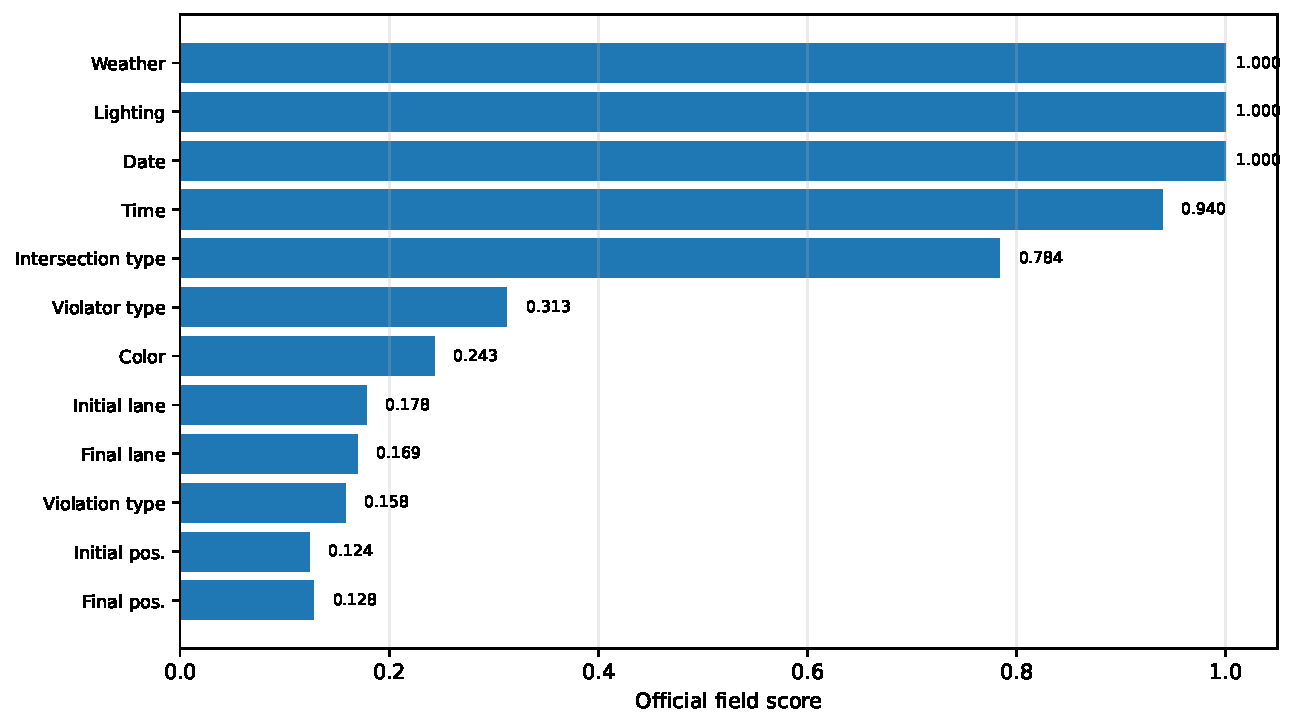
\includegraphics[width=0.90\textwidth]{fig_fetv_fields.pdf}
\caption{Official FETV field-level results. Global and overlay-associated attributes score highest, whereas violator-centric geometry and violation fields score lower, motivating the coupling analysis in \Cref{sec:fetvcase}.}
\label{fig:fetvfields}
\end{figure}


\begin{table}[t]
\caption{Complete PSI-VQA public leaderboard. KoreaDrive denotes Team 277, registered on the evaluation portal as ``Korea Drive.''}
\label{tab:psileader}
\centering
\scriptsize
\begin{tabular}{@{}clrrrrr@{}}
\toprule
Rank & Team & Final & BCQ mF1 & OpenQA & MCQ Acc. & T-mIoU \\
\midrule
1 & UWIPL\_ETRI & 70.64 & 0.7084 & 0.5833 & 0.7912 & 0.7427 \\
2 & MobilityAI & 69.07 & 0.6136 & 0.6674 & 0.7912 & 0.6906 \\
3 & OptimAI & 65.55 & 0.6464 & 0.5846 & 0.7253 & 0.6656 \\
4 & MR-CAS & 64.42 & 0.5934 & 0.6389 & 0.7692 & 0.5751 \\
5 & KoreaDrive & \textbf{57.04} & \textbf{0.5045} & \textbf{0.6019} & \textbf{0.6044} & \textbf{0.5708} \\
6 & SMART Lab & 54.24 & 0.5796 & 0.5793 & 0.6154 & 0.3955 \\
7 & Team KODE & 53.15 & 0.5796 & 0.5793 & 0.5714 & 0.3955 \\
\bottomrule
\end{tabular}
\end{table}


\Cref{tab:tar} reports every TAR component. The nine scored components average 0.42561 and reconstruct the official mean. MCQ-OE denotes multiple-choice open-ended questions. The strongest component was MCQ-OE BERTScore-F1 (0.7664). On the separate TAR General board, the organizers publish 13 baseline entries. The baseline labeled Qwen3-VL-8B-Instruct scores 0.3143, 0.1113 below KoreaDrive's 0.4256; the Qwen3-VL-32B-Instruct baseline scores 0.2875, 0.1381 below. KoreaDrive's score is numerically above 11 of the 13 organizer baselines, while Cosmos3-Super is the strongest baseline at 0.5729. The export exposes only model labels for these baseline rows, not their exact weight revisions, precision, frame policy, prompts, or decoding. We therefore treat them as external same-model-label references, not as same-checkpoint controls or evidence that any particular KoreaDrive component caused the margin.


\subsection{Fisheye Traffic Violation Understanding (FETV)}
\Cref{tab:fetvleader} is the complete eight-team public board. FETV is the strongest competitive result among our three Track 3 leaderboards: KoreaDrive placed 3rd of 8 with a final score of 0.4634. Its description score was second-highest and 0.0067 above the winning team's description score, while the remaining gap was concentrated in categorical violator-centric fields.


The field scores in \Cref{fig:fetvfields} split into global or overlay-associated attributes and violator-centric geometry. Weather, lighting, date, time, and intersection type achieve the highest scores, while violation type, position, and lane remain lower. Between submitted versions v8 and v11, 67/200 clips changed at least one violator-dependent field; in 51 clips the violation type and all six dependent violator fields changed together. This coordinated movement motivates treating the lower-scoring fields as a coupled violator-record decision rather than as independent field predictions.


\subsection{Pedestrian Situated Intent VQA (PSI-VQA)}
\Cref{tab:psileader} is the complete seven-team public board. KoreaDrive's OpenQA score is 0.6019, above the top-ranked team's 0.5833, and temporal mIoU is 0.5708, within 0.0043 of the fourth-place team. BCQ and MCQ account for most of the remaining gap, motivating the target-grounding and output-control analyses in \Cref{sec:controlled}.


\section{Controlled Component Analysis}\label{sec:controlled}
\subsection{Temporal localization and calibration}\label{sec:temporal}
This analysis corresponds to the PSI-VQA \emph{output / post-processing} block highlighted in \Cref{fig:system}: the duration-prior threshold and normalized interval endpoints are the fitted control parameters. We evaluate temporal prediction on the 227 labelled PSI training clips using five video-grouped splits (seed 42). Every parameterized baseline is fitted only on the training half of each split and evaluated on the held-out half. The duration threshold search is $T\in\{6,\ldots,14\}$~s; normalized interval endpoints use a 0.02 grid; centered-window width uses a 0.01 grid; the objective is mean training-fold IoU.

\Cref{fig:temporal} shows that the video-aware VLM configuration captures substantial temporal signal beyond random intervals (0.4617 vs. 0.2741). Simple fitted temporal priors provide additional localization strength: the centered window reaches 0.5200, the global mean interval 0.5369, the VLM-prior blend 0.5495, and the held-out duration-stratified prior 0.5566. The shipped constants score 0.5724 on the same splits but were fitted on all 227 windows; the 0.0158 difference from the held-out 0.5566 estimates fit optimism. Across folds, the short-clip lower endpoint remains 0.28--0.32 and the long-clip lower endpoint 0.20--0.22, while the selected threshold varies from 7 to 12~s because the short stratum contains only about 30 clips. The result identifies calibration as a meaningful component of the deployed system rather than attributing temporal localization solely to the VLM.

\begin{figure}[t]
\centering
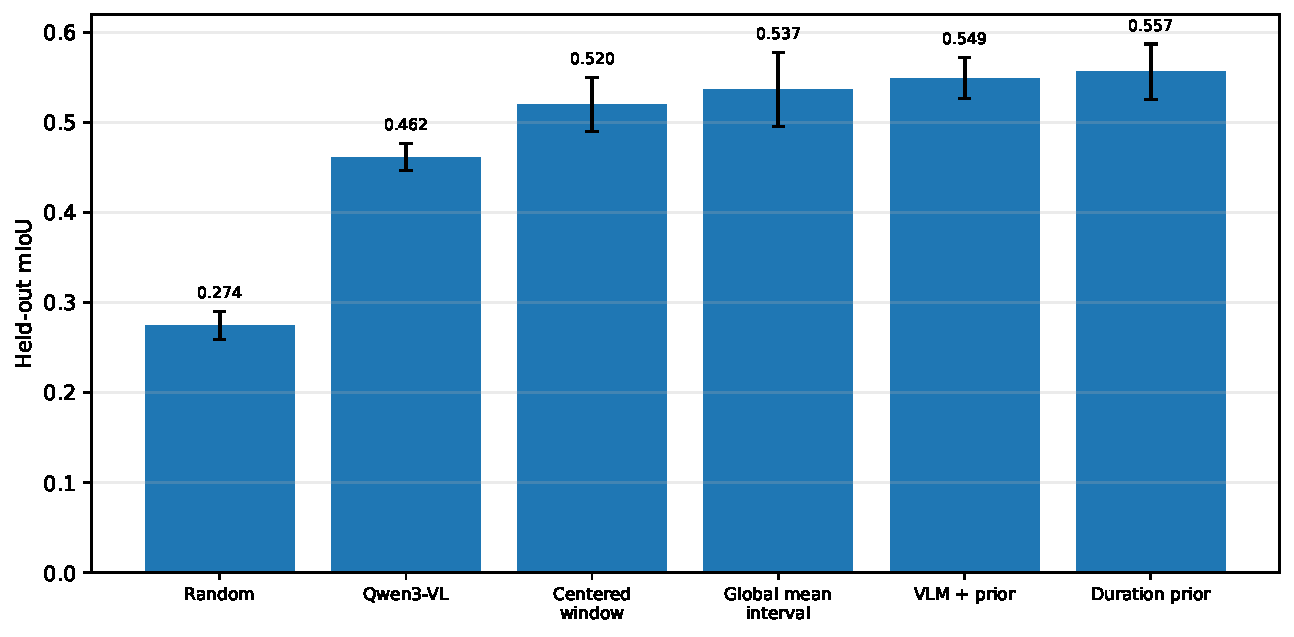
\includegraphics[width=0.88\textwidth]{fig_psi_temporal.pdf}
\caption{PSI temporal localization on five video-grouped splits (mean with standard-deviation error bars). The video-aware Qwen3-VL configuration improves substantially over random intervals, while fitted metadata priors provide stronger localization on these held-out splits; this is the temporal-calibration control highlighted in Fig.~1. The shipped constants fitted on all 227 intervals (0.5724) are omitted because they are not held out.}
\label{fig:temporal}
\end{figure}

\subsection{Target grounding in PSI multiple choice}
This analysis corresponds to the PSI-VQA \emph{prompt program} block highlighted in \Cref{fig:system}: only the target-grounding instruction is changed. We compare prompt programs on the same held-out items with the same model identifier, weight revision, precision, frame budget, and decoding settings. The 24 items answered in all conditions form a paired subset. \Cref{tab:prompt} shows a task-dependent effect. The generic Track 3 MCQ prompt reaches 8/24 against 3/24 for the shipped routed prompt. Adding an explicit instruction to re-locate the red-boxed target pedestrian raises the routed configuration to 9/24 and wins all six discordant items against the shipped routed prompt ($p=0.0312$). The box-aware configuration is statistically indistinguishable from the generic prompt at this sample size. These results identify explicit target grounding as the material control change, rather than routing being harmful in itself.

\begin{table}[t]
\caption{Controlled PSI MCQ prompt-program ablation on 24 paired items. Only the target-grounding instruction changes between the routed configurations.}
\label{tab:prompt}
\centering
\small
\begin{tabularx}{\textwidth}{@{}Yrr@{}}
\toprule
Prompt program & Accuracy & Paired comparison \\
\midrule
Generic Track 3 MCQ (no task routing) & 8/24 (0.3333) & -- \\
Shipped \texttt{psi\_mcq} routed prompt & 3/24 (0.1250) & Generic wins 5--0, $p=0.0625$ \\
Routed + explicit red-box re-location & 9/24 (0.3750) & Beats routed 6--0, $p=0.0312$ \\
\bottomrule
\end{tabularx}
\end{table}

\subsection{FETV output-contract and timestamp transition}
The FETV marker in \Cref{fig:system} denotes a historical submission-artifact comparison rather than a one-factor ablation. Between submitted artifacts \texttt{v6\_fewshot} and \texttt{v7}, the organizer-scored result rises from 0.4238 to 0.4584. The ten non-temporal structured fields---violation type, violator type, color, both positions, both lanes, intersection type, weather, and lighting---are byte-identical. Date accuracy changes from 0.995 to 1.000, time accuracy from 0.79 to 0.94, and the description score from 0.3645 to 0.4209. At the artifact level, 0/200 descriptions in \texttt{v6\_fewshot} and 200/200 in \texttt{v7} use the deterministic \texttt{On <date> at <time>,} opener, while only 37/200 time values remain unchanged.

Because the final metric averages description score and categorical mean, the description change contributes 0.0282 and the categorical half contributes 0.0065, reconstructing a 0.0347 increase versus the reported 0.0346 after rounding. Thus approximately 81\% of this transition lies in the description half. Two components changed together, so the comparison supports only a joint association with deterministic output formatting and timestamp handling; it does not isolate either component and provides no prompt-only attribution.

\subsection{Sampling and scorer sensitivity}
The TAR comparison corresponds to the \emph{frame policy} block highlighted in \Cref{fig:system}. Timestamp-aware TAR sampling changes accuracy from 15/25 to 16/25 on the same questions. The matched comparison is directionally positive but too small to support a strong sampling claim. For PSI OpenQA, video-grouped five-fold selection finds two cues robust across four plausible metric variants, while the held-out local estimate of 0.7816 under one-to-one macro matching is higher than the official 0.6019. The gap quantifies the importance of validating against the organizer scorer rather than relying on a local reimplementation.

A historical PSI comparison provides a complementary check. From submission v6 to v7, only the 126 OpenQA rows changed: Cue-F1 increased from 0.5970 to 0.6019 while all other components remained identical, and the final score increased by 0.12 points. This clean portal comparison confirms that the local cross-validation projection of 4.5--7.5 points was optimistic and reinforces the scorer-sensitivity result above.

\subsection{Development-time adapter study}
A small QLoRA adapter was trained on a BCQ/MCQ subset of the released TAR annotations and evaluated on a local proxy that excluded its training examples. The adapter produced 49 correct answers over 77 successfully evaluated items (0.636). The frozen-backbone result for that exact sample was not preserved; the nearest surviving baseline used a different sample together with few-shot prompting and five-sample self-consistency. Because a matched control is unavailable, the experiment cannot establish a fine-tuning gain. No fine-tuned checkpoint contributed to TAR, FETV, or PSI-VQA submissions, so the result is reported as development provenance rather than as a controlled ablation.

\section{Diagnostic Case Studies and Cross-Domain Interpretation}
\subsection{FETV: coupled violator-centric fields}\label{sec:fetvcase}
The submitted system predicts one complete FETV record in one generation, coupling
violator selection with violation type, vehicle attributes, position, and lane. In clip
019\_004.mp4, one system version predicts no violation and \texttt{na} for all dependent
fields; a later version predicts \texttt{red\_light}, a yellow car, Top-Left to Middle-Center
motion, and lanes 1 to 2, while date, time, weather, lighting, and intersection
type remain identical. Across the test set, 51 clips change the complete violator-
dependent block together, while the remaining 149 clips show no such coordinated
change. This observed co-movement is consistent with a single upstream
violator/event decision governing several downstream fields, though the current
evidence does not isolate the mechanism.

\begin{figure}[t]
\centering
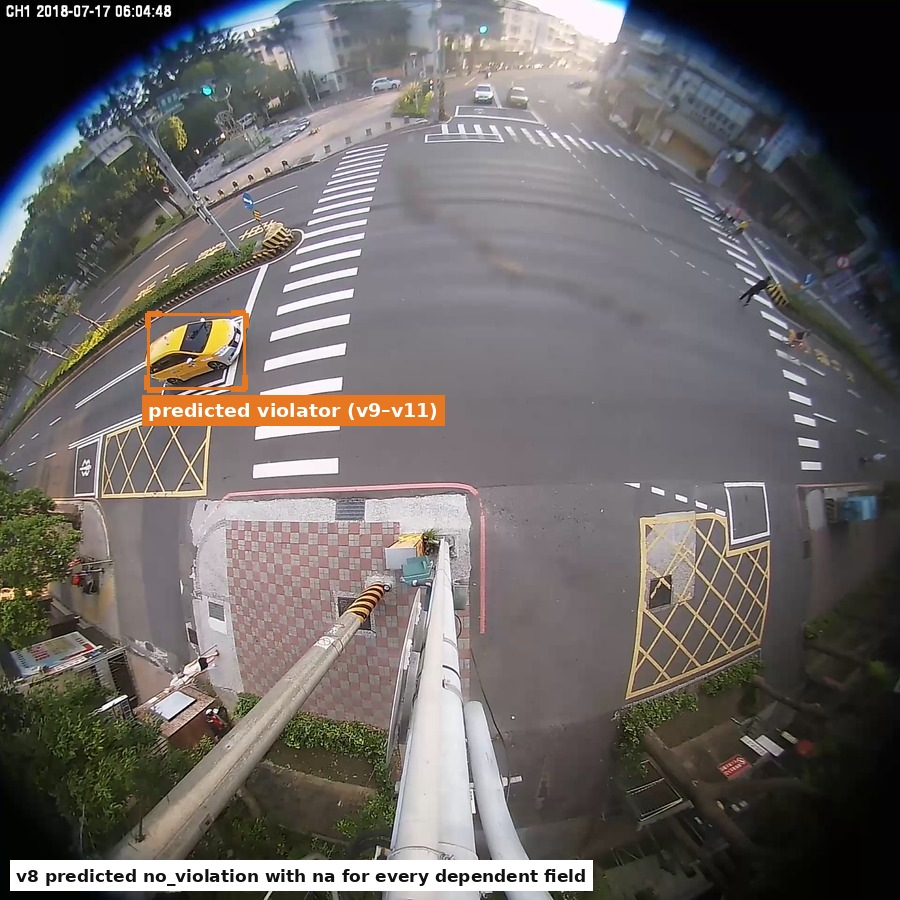
\includegraphics[width=0.72\textwidth,trim=0 450 245 0,clip]{frames/fetv_019_004_annotated.jpg}
\caption{FETV diagnostic from public clip \texttt{019\_004.mp4}~\cite{aicity2026track3,fisheye8k}. The orange box marks the yellow car designated as the violator by submitted artifacts v9--v11; v8 instead predicts \texttt{no\_violation} and \texttt{na} for every dependent field. The box visualizes a system prediction, not ground truth; scored-subset labels are not public. Global scene attributes remain unchanged across these artifacts.}
\label{fig:fetvcase}
\end{figure}

\subsection{PSI: answer-contract failure after correct target grounding}
The worked case in \Cref{fig:case} separates target perception from answer control. The model correctly follows the red-boxed target pedestrian and describes the ground-truth option, but the routed elimination procedure mis-negates that evidence, repeats prior reasoning, and reaches the token limit before emitting the required final letter. The submission builder then substitutes the type-correct fallback A. The visual evidence is therefore useful, while the benchmark answer is determined by the downstream reasoning and output contract.

\begin{figure}[t]
\centering
\footnotesize
\setlength{\fboxsep}{5pt}
\begin{tabularx}{\textwidth}{@{}L{0.20\textwidth}Y@{}}
\toprule
Held-out item & \texttt{e686c1a878234aa1}, question: why the pedestrian might \emph{not} intend to cross \\
\midrule
Ground truth D & ``Pedestrian was standing still and not moving into the roadway; pedestrian remained on the sidewalk.'' \\
\midrule
Model evidence & ``The pedestrian ... is standing on the sidewalk at the edge of the road ... does not move into the roadway; they remain on the sidewalk throughout the clip.'' \\
\midrule
Observed behavior & The elimination step mis-negates the supported option, repeats prior sentences, and is truncated before \texttt{Final answer: D}. No letter is parseable. \\
\midrule
Submission effect & The parser substitutes the type-correct fallback \texttt{A}, so the answer-contract issue appears in the submission as an ordinary wrong answer. \\
\bottomrule
\end{tabularx}
\caption{Worked PSI MCQ diagnostic case. The visual evidence and target pedestrian are correctly identified, but the reasoning/output-control path does not emit the required final letter before truncation. PSI-VQA frames are not redistributed under the benchmark data terms.}
\label{fig:case}
\end{figure}

\subsection{Cross-domain interpretation}
The scored submission artifacts record the same model identifier, precision, and weight revision, so TAR, FETV, and PSI-VQA were scored under one frozen checkpoint. The strongest outputs appear in free-form descriptions, cue-style observations, and global scene attributes. FETV shows that violator-centric geometry is where stronger explicit structure would help most, while the PSI case shows that correct target perception can still require tighter answer control. Across domains, the shared VLM therefore provides a reusable semantic backbone, and the dominant control need shifts among target grounding, geometry, temporal calibration, and format compliance.

\section{Design Implications and Exploratory Prototypes}
Neither prototype was deployed or scored. The exploratory FETV design would select a violator from tracked boxes, lane polygons, event flags, scene metadata, and overlay text, but lacks end-to-end perception modules. The PSI red-box prompt was evaluated only in Section~6.2 (9/24 vs.\ 3/24 shipped, $p=0.0312$; statistically indistinguishable from the 8/24 generic prompt) and was not deployed. Together, they motivate combining tracking and geometry, constrained decoding, and VLM semantics.


\section{Reproducibility, Efficiency, Limitations, and Ethics}
\paragraph{Artifacts and provenance.}
The public repository\footnote{\url{https://github.com/hwkim3330/aicity2026}; artifact, reproduction, camera-ready consistency records, and FETV figure assets were checked against commit \texttt{d100b24}.} contains the three scored submission artifacts, prompts, environment files, validators, hashes, leaderboard exports, controlled analyses, and case descriptions. All three scored Qwen3-VL runs use the recovered Hub revision \texttt{0c351dd01ed87e9c1b53cbc748cba10e6187ff3b}. Exact PSI byte reproduction remains limited by unseeded five-sample voting for 55 BCQ records. FETV has a different provenance boundary: the released command reproduces the single-pass configuration rather than the final v11 chain. Re-running that configuration on the public clips matches \texttt{v6\_fewshot} on 1742/2600 fields (67.0\%). Two identical reruns agree bit-for-bit on all 13 fields for all 200 clips, showing that the residual difference is systematic rather than run-to-run variance. Six tested explanations---nondeterminism, cuDNN pinning, clip encoding, frame sampling, few-shot exemplars, and the NumPy upgrade---were ruled out; the repository does not establish a remaining cause. The v10-to-v11 description step is recovered exactly, while intermediate FETV code states remain a documented provenance gap. Exploratory \texttt{psi\_vqa\_submission\_v8\_final.csv} and \texttt{fetv\_structured\_pipeline.py} are explicitly excluded from leaderboard results.

\paragraph{Data use.}
The scored submissions and controlled analyses use only the AI City Challenge 2026 Track 3 benchmark data, released annotations, and benchmark-provided metadata under the applicable benchmark and source-dataset access terms; no private data or private models are used. Figure~\ref{fig:fetvcase} reproduces one downscaled frame from a public FETV clip with source attribution and marks a submitted system prediction rather than adding a ground-truth label. No PSI-VQA or TAR frames are redistributed, and access to those videos remains through the original benchmark or source-dataset providers.

\paragraph{Efficiency.}
Original challenge runs did not log runtime or peak memory. A reproduction run on 2026-08-03 used one RTX 3090 24~GB (PyTorch 2.10.0, Transformers 5.13.0). On 227 PSI temporal items, model loading took 18.7~s, inference 469.3~s (2.07~s/item), and peak allocated VRAM was 16.78~GiB. These measurements support the single-consumer-GPU claim but should not be read as timings of the scored runs.

\paragraph{Limitations.}
No task-specific parameter update or adapter generated the scored submissions. The unmatched TAR QLoRA study cannot support a fine-tuning claim; prompt samples are small, some development used sequential leaderboard feedback, and local metrics can differ from organizer scorers. The temporal prior is benchmark-specific. Some intermediate FETV v11 code states were not committed, despite documented artifact integrity and exact recovery of the v10-to-v11 description step. Finally, post-hoc parsing can conceal answer-contract errors; token-level constrained decoding is a direct next step.

\paragraph{Ethics.}
Traffic and pedestrian video can reveal personal behavior and create privacy, bias, and misuse risks. We use data only under benchmark and source-dataset terms, do not redistribute restricted clips, and do not manually label test data. Pedestrian-intent outputs are uncertain decision-support signals, not ground truth about a person's future action.

\section{Conclusion}
KoreaDrive uses one frozen Qwen3-VL-8B-Instruct backbone across TAR, FETV, and PSI-VQA with task-specific inference controls and no parameter updates. Controlled analyses identify explicit target grounding and temporal calibration as material controls, while FETV exposes the need for stronger violator-centric consistency. The cases further separate semantic evidence from answer-contract compliance. The resulting design is hybrid: the frozen VLM supplies reusable semantics, and explicit grounding, geometry, calibration, and constrained output provide benchmark-specific structure.

\paragraph{Acknowledgements.}
This work was supported by the Ministry of Science and ICT, the Institute of Information \& Communications Technology Planning \& Evaluation (IITP) grant funded by the Korea government (No.~RS-2025-02283230, Development of Autonomous Cooperative Driving Technology Based on Seamless Communication of Heterogeneous V2X for Autonomous Driving), and by the Korea Planning \& Evaluation Institute of Industrial Technology (KEIT) grant funded by the Ministry of Trade, Industry and Resources (MOTIR) (No.~RS-2024-00404601).

\bibliographystyle{splncs04}
\bibliography{main}
\end{document}
